\documentclass[bachelor, och, otchet]{SCWorks}
% параметр - тип обучения - одно из значений:
%    spec     - специальность
%    bachelor - бакалавриат (по умолчанию)
%    master   - магистратура
% параметр - форма обучения - одно из значений:
%    och   - очное (по умолчанию)
%    zaoch - заочное
% параметр - тип работы - одно из значений:
%    referat    - реферат
%    coursework - курсовая работа (по умолчанию)
%    diploma    - дипломная работа
%    pract      - отчет по практике
%    pract      - отчет о научно-исследовательской работе
%    autoref    - автореферат выпускной работы
%    assignment - задание на выпускную квалификационную работу
%    review     - отзыв руководителя
%    critique   - рецензия на выпускную работу
% параметр - включение шрифта
%    times    - включение шрифта Times New Roman (если установлен)
%               по умолчанию выключен
\usepackage[T2A]{fontenc}
\usepackage[utf8]{inputenc}
\usepackage{graphicx}

\usepackage[sort,compress]{cite}
\usepackage{amsmath}
\usepackage{amssymb}
\usepackage{amsthm}
\usepackage{fancyvrb}
\usepackage{longtable}
\usepackage{array}
\usepackage[english,russian]{babel}
\usepackage{minted}

\usepackage{tempora}


\usepackage[colorlinks=false]{hyperref}


\newcommand{\eqdef}{\stackrel {\rm def}{=}}

\newtheorem{lem}{Лемма}


\begin{document}

\chair{Кафедра теоретических основ компьютерной безопасности и криптографии}


\title{Классификация бинарных отношений и системы замыканий}


\course{3}

\group{331}


\department{факультета КНиИТ}

\napravlenie{10.05.01 "--- Компьютерная безопасность}

% Для студентки. Для работы студента следующая команда не нужна.
%\studenttitle{Студентки}

% Фамилия, имя, отчество в родительном падеже
\author{Никитина Арсения Владимировича}

% Заведующий кафедрой
% \chtitle{доцент, к.\,ф.-м.\,н.} % степень, звание
% \chname{С.\,В.\,Миронов}

%Научный руководитель (для реферата преподаватель проверяющий работу)
% \satitle{доцент, к.\,ф.-м.\,н.} %должность, степень, звание
\satitle{ассистент}
\saname{Р.\,А.\,Фарахутдинов}

% Руководитель практики от организации (только для практики,
% для остальных типов работ не используется)
% \patitle{к.\,ф.-м.\,н., доцент}
% \paname{Д.\,Ю.\,Петров}

% Семестр (только для практики, для остальных
% типов работ не используется)
% \term{2}

% Наименование практики (только для практики, для остальных
% типов работ не используется)
% \practtype{учебная}

% Продолжительность практики (количество недель) (только для практики,
% для остальных типов работ не используется)
% \duration{2}

% Даты начала и окончания практики (только для практики, для остальных
% типов работ не используется)
% \practStart{01.07.2016}
% \practFinish{14.07.2016}

% Год выполнения отчета
\date{2022}

\maketitle

% Включение нумерации рисунков, формул и таблиц по разделам
% (по умолчанию - нумерация сквозная)
% (допускается оба вида нумерации)
%\secNumbering


\tableofcontents

% Раздел "Обозначения и сокращения". Может отсутствовать в работе
% \abbreviations
% \begin{description}
%     \item ... "--- ...
%     \item ... "--- ...
% \end{description}

% Раздел "Определения". Может отсутствовать в работе
%\definitions

% Раздел "Определения, обозначения и сокращения". Может отсутствовать в работе.
% Если присутствует, то заменяет собой разделы "Обозначения и сокращения" и "Определения"
%\defabbr


% Раздел "Введение"

\intro

Существует определенная классификация бинарных отношений в зависимости от их свойств. Задачей данной работы является рассмотрение 
основных свойств бинарных отношений, а также их классификация. В зависимости от класса бинарного отношения, на нем можно определить замыкание: относительно рефлексивности,
симметричности и транзитивности. Для этого требуется понимать, каким образом происходит классификация отношений в зависимости от множеств, которыми они могут задаваться.



\section{Основные виды бинарных отношений и алгоритмы их классификации}

Бинарное отношение $\rho \subset A \times A$ называется:

\begin{enumerate}
    \item \textit{рефлексивным}, если $(a,a) \in \rho$ $\forall a \in A$\
    
    \item \textit{симметричным}, если $(a,b) \in \rho \Rightarrow (b,a) \in \rho$
    
    \item \textit{антисимметричным}, если $(a,b) \in \rho$ и $(b,a) \in \rho \Rightarrow a = b$
    \item \textit{транзитивным}, если  $(a,b) \in \rho$ и $(b,c) in \rho \Rightarrow (a,c) \in \rho$ 
    
    % \begin{figure}[H]
    %     \centering      %размер рисунка       здесь находится название файла рисунка, без указания формата
    %     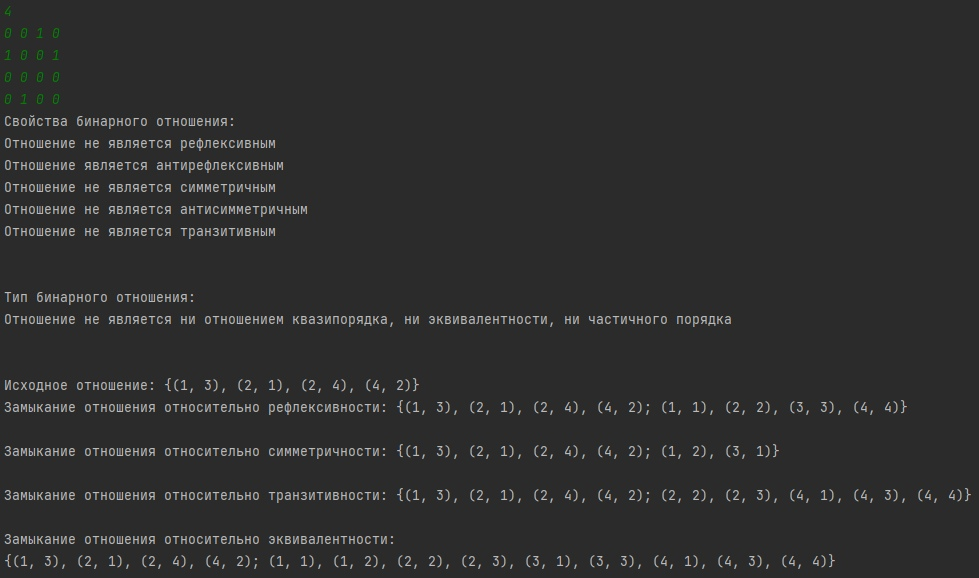
\includegraphics[width=1\textwidth]{1}
    %     \label{fig:image1}
    % \end{figure}
\end{enumerate}
% После введения — серии \section, \subsection и т.д.
% $\displaystyle f(y) = \frac{\sin x_0^3}{6}$

% \begin{equation*}
%     x = 4
%     \text{ "= лучшая формула в мире}
% \end{equation*}

% \begin{figure}[h!]
%     \centering
%     \includegraphics[scale=0.2,]{}
% \end{figure}


% \begin{tabular*}{}[]{}
    
% \end{tabular*}


% \begin{minted}[linenos,breaklines=true, fontsize=\small, style=bw]{python}
    
% \end{minted}
% \inputminted
% Раздел "Заключение"
\conclusion

%Библиографический список, составленный вручную, без использования BibTeX
%
%\begin{thebibliography}{99}
%  \bibitem{Ione} Источник 1.
%  \bibitem{Itwo} Источник 2
%\end{thebibliography}
\cite{firstmetka}
%Библиографический список, составленный с помощью BibTeX
%
\bibliographystyle{gost780uv}
\inputencoding{cp1251}
\bibliography{thesis}
\inputencoding{utf8}
% % При использовании biblatex вместо bibtex
%\printbibliography

% Окончание основного документа и начало приложений
% Каждая последующая секция документа будет являться приложением
\appendix

\end{document}